\documentclass{beamer}
\usepackage[utf8]{inputenc}

\usetheme{Madrid}
\usecolortheme{default}
\usepackage{amsmath,amssymb,amsfonts,amsthm}
\usepackage{txfonts}
\usepackage{tkz-euclide}
\usepackage{listings}
\usepackage{adjustbox}
\usepackage{array}
\usepackage{tabularx}
\usepackage{gvv}
\usepackage{lmodern}
\usepackage{circuitikz}
\usepackage{tikz}
\usepackage{graphicx}

\setbeamertemplate{page number in head/foot}[totalframenumber]

\usepackage{tcolorbox}
\tcbuselibrary{minted,breakable,xparse,skins}

\definecolor{bg}{gray}{0.95}
\DeclareTCBListing{mintedbox}{O{}m!O{}}{%
  breakable=true,
  listing engine=minted,
  listing only,
  minted language=#2,
  minted style=default,
  minted options={%
    linenos,
    gobble=0,
    breaklines=true,
    breakafter=,,
    fontsize=\small,
    numbersep=8pt,
    #1},
  boxsep=0pt,
  left skip=0pt,
  right skip=0pt,
  left=25pt,
  right=0pt,
  top=3pt,
  bottom=3pt,
  arc=5pt,
  leftrule=0pt,
  rightrule=0pt,
  bottomrule=2pt,
  toprule=2pt,
  colback=bg,
  colframe=orange!70,
  enhanced,
  overlay={%
    \begin{tcbclipinterior}
    \fill[orange!20!white] (frame.south west) rectangle ([xshift=20pt]frame.north west);
    \end{tcbclipinterior}},
  #3,
}
\lstset{
    language=C,
    basicstyle=\ttfamily\small,
    keywordstyle=\color{blue},
    stringstyle=\color{orange},
    commentstyle=\color{green!60!black},
    numbers=left,
    numberstyle=\tiny\color{gray},
    breaklines=true,
    showstringspaces=false,
}

\title{5.5.17}
\date{September 27,2025}
\author{EE25BTECH11065-Yoshita J}

\begin{document}

\frame{\titlepage}

\begin{frame}{Question}
If 
\[
\vec{A} = 
\myvec{
1 & 1 & 1\\
0 & 1 & 3\\
1 & -2 & 1
},
\]
find \( \vec{A}^{-1} \) using elementary row transformations. Hence, solve the system:
\begin{align*}
x + y + z &= 6\\
y + 3z &= 11\\
x - 2y + z &= 0
\end{align*}
\end{frame}

\begin{frame}{Theoretical Solution}
\begin{align}
\vec{A} = 
\begin{pmatrix}
1 & 1 & 1\\
0 & 1 & 3\\
1 & -2 & 1
\end{pmatrix}
\end{align}

The augmented matrix is:
\begin{align}
\augvec{3}{3}{
1 & 1 & 1 & 1 & 0 & 0 \\
0 & 1 & 3 & 0 & 1 & 0 \\
1 & -2 & 1 & 0 & 0 & 1
}
\end{align}
\end{frame}

\begin{frame}{Theoretical Solution}
Row operations:

\begin{align}
R_3 \to R_3 - R_1 &\Rightarrow 
\augvec{3}{3}{
1 & 1 & 1 & 1 & 0 & 0 \\
0 & 1 & 3 & 0 & 1 & 0 \\
0 & -3 & 0 & -1 & 0 & 1
}
\\
R_3 \to R_3 + 3R_2 &\Rightarrow 
\augvec{3}{3}{
1 & 1 & 1 & 1 & 0 & 0 \\
0 & 1 & 3 & 0 & 1 & 0 \\
0 & 0 & 9 & -1 & 3 & 1
}
\\
R_3 \to \frac{1}{9}R_3 &\Rightarrow 
\augvec{3}{3}{
1 & 1 & 1 & 1 & 0 & 0 \\
0 & 1 & 3 & 0 & 1 & 0 \\
0 & 0 & 1 & -\frac{1}{9} & \frac{1}{3} & \frac{1}{9}
}
\end{align}
\end{frame}

\begin{frame}{Theoretical Solution}
\begin{align}
R_1 \to R_1 - R_3,\quad R_2 \to R_2 - 3R_3 &\Rightarrow 
\augvec{3}{3}{
1 & 1 & 0 & \frac{10}{9} & -\frac{1}{3} & -\frac{1}{9} \\
0 & 1 & 0 & \frac{1}{3} & 0 & -\frac{1}{3} \\
0 & 0 & 1 & -\frac{1}{9} & \frac{1}{3} & \frac{1}{9}
}
\\
R_1 \to R_1 - R_2 &\Rightarrow 
\augvec{3}{3}{
1 & 0 & 0 & \frac{7}{9} & -\frac{1}{3} & \frac{2}{9} \\
0 & 1 & 0 & \frac{1}{3} & 0 & -\frac{1}{3} \\
0 & 0 & 1 & -\frac{1}{9} & \frac{1}{3} & \frac{1}{9}
}
\end{align}
\end{frame}

\begin{frame}{Theoretical Solution}

As the left block becomes identity, the right block is \( \vec{A}^{-1} \):

\begin{align}
\vec{A}^{-1} = 
\myvec{
\frac{7}{9} & -\frac{1}{3} & \frac{2}{9}\\
\frac{1}{3} & 0 & -\frac{1}{3}\\
-\frac{1}{9} & \frac{1}{3} & \frac{1}{9}
}
\end{align}

Now solving: \quad \( \vec{x} = \vec{A}^{-1} \vec{b} \), where
\[
\vec{b} = 
\myvec{
6\\
11\\
0
}
\]


\end{frame}

\begin{frame}{Theoretical Solution}
\begin{align*}
\vec{x} = 
\myvec{
\frac{7}{9} & -\frac{1}{3} & \frac{2}{9}\\
\frac{1}{3} & 0 & -\frac{1}{3}\\
-\frac{1}{9} & \frac{1}{3} & \frac{1}{9}
}
\myvec{
6\\
11\\
0
}
=
\myvec{
1\\
2\\
3
}
\end{align*}

\textbf{Final Answer:}
\begin{align*}
\boxed{x = 1,\quad y = 2,\quad z = 3}
\end{align*}

\end{frame}












\begin{frame}[fragile]
    \frametitle{C Code}

    \begin{lstlisting}
#include <stdio.h>

void inverse3x3(double A[3][3], double inv[3][3]);
void multiply3x3_3x1(double A[3][3], double B[3], double result[3]);
void printVector(double v[3]);

int main() {
    double A[3][3] = {
        {1, 1, 1},
        {0, 1, 3},
        {1, -2, 1}
    };
    double b[3] = {6, 11, 0};
    double A_inv[3][3];
    double x[3];

    
    \end{lstlisting}
\end{frame}

\begin{frame}[fragile]
    \frametitle{C Code}
    \begin{lstlisting}
inverse3x3(A, A_inv);
    multiply3x3_3x1(A_inv, b, x);

    printf("Solution:\n");
    printf("x = %.6lf\n", x[0]);
    printf("y = %.6lf\n", x[1]);
    printf("z = %.6lf\n", x[2]);

    return 0;
}
void inverse3x3(double A[3][3], double inv[3][3]) {
    double det =
          A[0][0]*(A[1][1]*A[2][2] - A[1][2]*A[2][1])
        - A[0][1]*(A[1][0]*A[2][2] - A[1][2]*A[2][0])
        + A[0][2]*(A[1][0]*A[2][1] - A[1][1]*A[2][0]);

    if(det == 0) {
        printf("Matrix is singular, no inverse.\n");
        return;
    }

    double invDet = 1.0 / det;
    \end{lstlisting}
\end{frame}

\begin{frame}[fragile]
    \frametitle{C Code}
    \begin{lstlisting}
    inv[0][0] =  (A[1][1]*A[2][2] - A[1][2]*A[2][1]) * invDet;
    inv[0][1] = -(A[0][1]*A[2][2] - A[0][2]*A[2][1]) * invDet;
    inv[0][2] =  (A[0][1]*A[1][2] - A[0][2]*A[1][1]) * invDet;

    inv[1][0] = -(A[1][0]*A[2][2] - A[1][2]*A[2][0]) * invDet;
    inv[1][1] =  (A[0][0]*A[2][2] - A[0][2]*A[2][0]) * invDet;
    inv[1][2] = -(A[0][0]*A[1][2] - A[0][2]*A[1][0]) * invDet;

    inv[2][0] =  (A[1][0]*A[2][1] - A[1][1]*A[2][0]) * invDet;
    inv[2][1] = -(A[0][0]*A[2][1] - A[0][1]*A[2][0]) * invDet;
    inv[2][2] =  (A[0][0]*A[1][1] - A[0][1]*A[1][0]) * invDet;
}
   
    \end{lstlisting}
\end{frame}
\begin{frame}[fragile]
    \frametitle{C Code}
    \begin{lstlisting}


void multiply3x3_3x1(double A[3][3], double B[3], double result[3]) {
    for(int i = 0; i < 3; i++) {
        result[i] = 0;
        for(int j = 0; j < 3; j++) {
            result[i] += A[i][j] * B[j];
        }
    }
}
   
    \end{lstlisting}
\end{frame}

\begin{frame}[fragile]
    \frametitle{Python Code}
    \begin{lstlisting}
import numpy as np
import matplotlib.pyplot as plt
from mpl_toolkits.mplot3d import Axes3D

x_vals = np.linspace(-10, 10, 50)
y_vals = np.linspace(-10, 10, 50)
x, y = np.meshgrid(x_vals, y_vals)

z1 = 6 - x - y
z2 = (11 - y) / 3
z3 = 2*y - x

A = np.array([
    [1, 1, 1],
    [0, 1, 3],
    [1, -2, 1]
])
b = np.array([6, 11, 0])

    \end{lstlisting}
\end{frame}

\begin{frame}[fragile]
    \frametitle{Python Code}
    \begin{lstlisting}
intersection_point = np.linalg.solve(A, b)
px, py, pz = intersection_point

fig = plt.figure(figsize=(10, 8))
ax = fig.add_subplot(111, projection='3d')

ax.plot_surface(x, y, z1, alpha=0.5, color='red', label='Plane 1')
ax.plot_surface(x, y, z2, alpha=0.5, color='green', label='Plane 2')
ax.plot_surface(x, y, z3, alpha=0.5, color='blue', label='Plane 3')

ax.scatter(px, py, pz, color='black', s=100, label='Intersection Point')
ax.text(px, py, pz + 1, f"({px:.2f}, {py:.2f}, {pz:.2f})", color='black')
   
    \end{lstlisting}
\end{frame}

\begin{frame}[fragile]
    \frametitle{Python Code}
    \begin{lstlisting}
ax.text(6, -9, 8, "x + y + z = 6", color='red')
ax.text(-10, 9, (11 - 9)/3, "y + 3z = 11", color='green')
ax.text(-9, -9, 2*(-9) - (-9), "x - 2y + z = 0", color='blue')
ax.set_xlabel('X-axis')
ax.set_ylabel('Y-axis')
ax.set_zlabel('Z-axis')
ax.set_xlim(-10, 10)
ax.set_ylim(-10, 10)
ax.set_zlim(-10, 10)
ax.set_xticks(np.linspace(-10, 10, 5))
ax.set_yticks(np.linspace(-10, 10, 5))
ax.set_zticks(np.linspace(-10, 10, 5))

ax.grid(True)
ax.set_title('Intersection of Three Planes')
ax.legend()

plt.show()
    \end{lstlisting}
\end{frame}

\begin{frame}{Plot}
\begin{figure}[h!]
\begin{center}
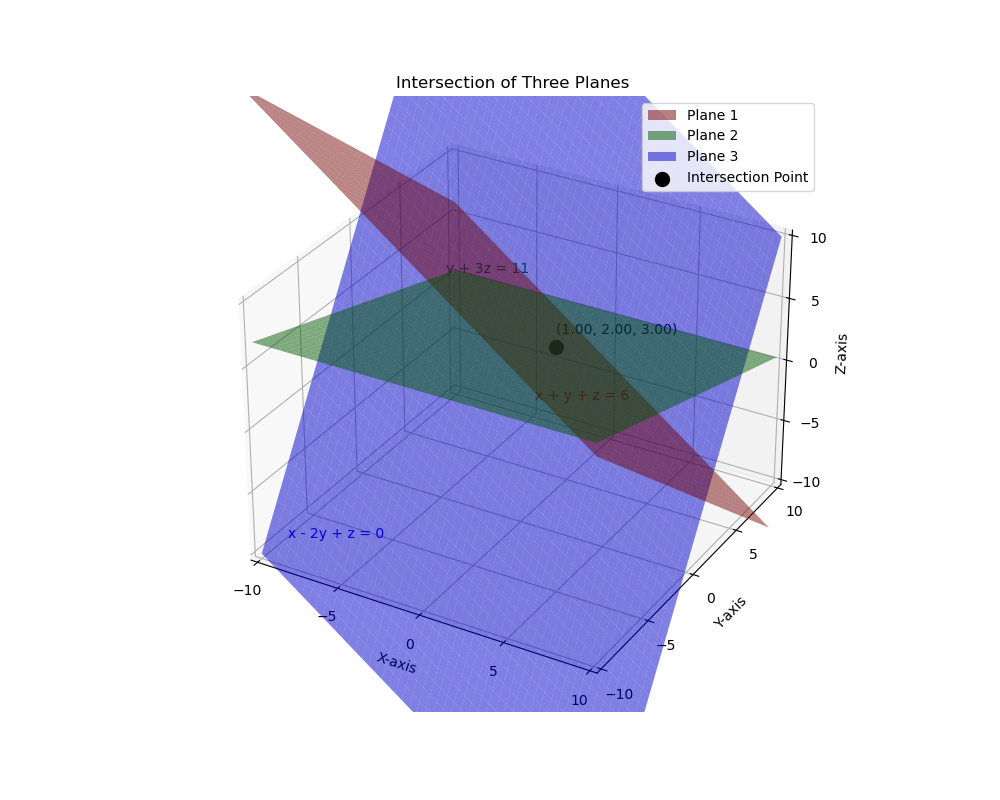
\includegraphics[width=\columnwidth]{figs/fig.png}
\end{center}
\caption{A plane passing through point A with normal vector n.}
\label{fig:Fig.1}
\end{figure}
  
\end{frame}

\end{document}

